\documentclass[10pt]{beamer}

\setbeamertemplate{footline}[page number]

\usepackage{tikz}
\usepackage{tikz-cd}
\usepackage{wasysym}

\DeclareFontFamily{U}{wncyr}{}
\DeclareFontShape{U}{wncyr}{m}{n}{<->wncyr10}{}
\DeclareSymbolFont{cyr}{U}{wncyr}{m}{n}
\DeclareMathSymbol{\Sha}{\mathord}{cyr}{"58}

\newcommand{\abr}[1]{\langle #1 \rangle}

\begin{document}

\begin{frame}

\begin{center}

\vspace{1in}

\textbf{\large Ideal Class Groups \footnote{of number fields}}

\vspace{0.5in}

{\normalsize David Ang}

\vspace{0.25in}

{\small LSGNT}

{\scriptsize Short introductory talk}

{\tiny Wednesday, 6 October 2021}

\end{center}

\end{frame}

\begin{frame}[t]{Diophantine equations!}

Consider \emph{Mordell's equation}
$$ y^2 = x^3 + n, \qquad n \in \mathbb{Z}. $$
\begin{itemize}
\item<2-24> Consider $ y^2 = x^3 - 1 $.
\only<3-19>{Solution: $ (1, 0) $.
\only<4-19>{Claim: $ y = 0 $. \\}
\only<5-19>{Check: $ x $ odd.}
\only<6-19>{In $ \mathbb{Z}[i] $,
$$ \visible<6-19>{(y + i)(y - i) = x^3} \visible<7-19>{\overset{\mathrm{Nm}}{\implies} y \pm i \ \text{coprime}} \visible<14-19>{\overset{\text{UFD}}{\implies} y \pm i \ \text{cubes}.} $$%
}%
\only<8-13>{Otherwise
$$
\begin{tikzcd}[ampersand replacement=\&, column sep=-10, row sep=0]
{\visible<8-13>{p \mid y \pm i}} \& {\visible<9-13>{\overset{\mathrm{Nm}}{\implies}}} \& {\visible<9-13>{\mathrm{Nm}(p) \mid y^2 + 1 = x^3}} \& \& \\
{\visible<10-13>{\Downarrow}} \& \& \& {\visible<12-13>{\implies}} \& {\visible<12-13>{\mathrm{Nm}(p) = 1}} {\visible<13>{\ \text{\lightning}}} \\
{\visible<10-13>{p \mid 2i}} \& {\visible<11-13>{\overset{\mathrm{Nm}}{\implies}}} \& {\visible<11-13>{\mathrm{Nm}(p) \mid 4}} \& \&
\end{tikzcd}
$$
}%
\only<15-19>{Let
$$ y + i = (a + bi)^3 = a(a^2 - 3b^2) + b(3a^2 - b^2)i. $$
}%
\only<16-19>{Then $ b = \pm 1 $.
\begin{itemize}
\item<17-19> $ b = 1 \implies 3a^2 = 2 \ \text{\lightning} $
\item<18-19> $ b = -1 \implies 3a^2 = 0 \implies y = 0 \ \text{\checked} $
\end{itemize}
}
}%
\only<19-24>{Idea: use UF of $ \mathbb{Z}[i] $ and $ \mathrm{Nm} : \mathbb{Z}[i] \to \mathbb{N} $. \\}
\item<20-24> Consider $ y^2 = x^3 - 5 $.
\only<21-24>{In $ \mathbb{Z}[\sqrt{-5}] $,
$$ 6 = 2 \cdot 3 = (1 + \sqrt{-5}) \cdot (1 - \sqrt{-5}). $$
}%
\only<22-24>{However, on ideals,
$$ \abr{6} = \abr{2, 1 + \sqrt{-5}} \cdot \abr{2, 1 - \sqrt{-5}} \cdot \abr{3, 1 + \sqrt{-5}} \cdot \abr{3, 1 - \sqrt{-5}}. $$
}%
\only<23-24>{Furthermore, can define norm on ideals.}
\only<24>{Conclusion: consider ideals.}
\end{itemize}

\end{frame}

\begin{frame}[t]{The ideal class group...}

\only<1-8>{Let $ K $ be a number field,}
\only<2-8>{and let $ \mathcal{O}_K $ be its \emph{ring of integers},
$$ \mathcal{O}_K = \{x \in K \mid \exists f \in \mathbb{Z}[X] \ \text{monic}, \ f(x) = 0\}. $$
}
\only<3-8>{
\begin{examples}
\begin{itemize}
\item<3-8> $ K = \mathbb{Q} $ and $ \mathcal{O}_K = \mathbb{Z} $,
\item<4-8> $ K = \mathbb{Q}(i) $ and $ \mathcal{O}_K = \mathbb{Z}[i] $, or
\item<5-8> $ K = \mathbb{Q}(\sqrt{-3}) $ and $ \mathcal{O}_K = \mathbb{Z}[\omega] $ where $ \omega = \tfrac{1 + \sqrt{-3}}{2} $.
\end{itemize}
\end{examples}
}
\only<6-8>{
\begin{fact}
$ \mathcal{O}_K $ is a \emph{Dedekind domain}.
\only<7-8>{Every DD has UF into prime ideals.}
\only<8>{
$$
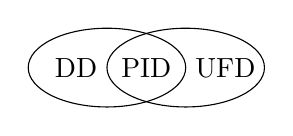
\begin{tikzpicture}
\draw (-0.5, 0) ellipse (1 and 0.5) node[left]{DD};
\draw (0.5, 0) ellipse (1 and 0.5) node[right]{UFD};
\draw (0, 0) node{PID};
\end{tikzpicture}
$$
}
\end{fact}
}
\only<9-15>{The \emph{ideal norm} is
$$ \mathrm{Nm}(I) = \#(\mathcal{O}_K / I), \qquad I \trianglelefteq \mathcal{O}_K. $$
}
\only<10-15>{
\begin{example}
If $ K = \mathbb{Q}(\sqrt{-5}) $, then $ \abr{2, 1 + \sqrt{-5}} \trianglelefteq \mathcal{O}_K $
\only<11-15>{has ideal norm}
\begin{align*}
\visible<11-15>{\mathrm{Nm}(\abr{2, 1 + \sqrt{-5}}) & = \#(\mathbb{Z}[\sqrt{-5}] / \abr{2, 1 + \sqrt{-5}}) \\}
\visible<12-15>{& = \#(\mathbb{Z}[X] / \abr{2, 1 + X, 5 + X^2}) \\}
\visible<13-15>{& = \#(\mathbb{F}_2[X] / \abr{1 + X, 1 + X^2})}
\visible<14-15>{= 2.}
\end{align*}
\end{example}
}
\only<15>{
\begin{fact}
$$ \mathrm{Nm}(I \cdot J) = \mathrm{Nm}(I)\mathrm{Nm}(J), \qquad \mathrm{Nm}(\abr{x}) = \mathrm{Nm}(x) = \prod_{\sigma : K \to \overline{K}} \sigma(x). $$
\end{fact}
}
\only<16-22>{Consider the set of non-zero \emph{fractional ideals} of $ \mathcal{O}_K $,
$$ \mathcal{I}(K) = \{x^{-1}I \subseteq K \mid x \in \mathcal{O}_K^\times, \ I \trianglelefteq \mathcal{O}_K\} \setminus \{\abr{0}\}. $$
}%
\only<17-22>{This is an abelian group under ideal multiplication, with identity $ \abr{1} $ and
$$ I^{-1} = \{x \in K \mid xI \subseteq \mathcal{O}_K\}, \qquad I \in \mathcal{I}(K). $$
}%
\only<18-22>{It has a subgroup of \emph{principal fractional ideals}
$$ \mathcal{P}(K) = \{\abr{x} \in \mathcal{I}(K) \mid x \in K^\times\} \le \mathcal{I}(K). $$
}%
\only<19-22>{The quotient is the \emph{ideal class group} $ \mathrm{Cl}(K) $.}
\only<20-22>{
\begin{theorem}
$ \mathrm{Cl}(K) $ is finite.
\end{theorem}
}
\only<21-22>{
\begin{proof}
\only<21-22>{\emph{Geometry of numbers} gives \emph{Minkowski's bound} $ \mathrm{M}_K \in \mathbb{R}_{> 0} $. \\}
\only<22>{Every $ [I] \in \mathrm{Cl}(K) $ has a representative $ I \trianglelefteq \mathcal{O}_K $ with $ \mathrm{Nm}(I) \le \mathrm{M}_K $.}
\end{proof}
}
\only<23-42>{
\begin{examples}
\begin{itemize}
\item<23-42> If $ K = \mathbb{Q}, \mathbb{Q}(i), \mathbb{Q}(\sqrt{-3}) $, then $ \mathrm{Cl}(K) = 1 $, since $ \mathcal{O}_K $ is a PID.
\item<24-42> If $ K = \mathbb{Q}(\sqrt{-5}) $, then $ \mathrm{Cl}(K) \ne 1 $, since $ \abr{2, 1 + \sqrt{-5}} \in \mathcal{I}(K) $ is not principal.
\only<25-42>{However $ \abr{2, 1 + \sqrt{-5}}^2 = \abr{2} $, so $ \mathbb{Z} / 2\mathbb{Z} \le \mathrm{Cl}(K) $.}
\only<26-42>{In fact $ \mathrm{Cl}(K) \cong \mathbb{Z} / 2\mathbb{Z} $, for instance $ \abr{3, 1 - \sqrt{-5}} = \abr{\tfrac{1 - \sqrt{-5}}{2}} \cdot \abr{2, 1 + \sqrt{-5}} $.}
\end{itemize}
\end{examples}
}
\only<27-42>{Consider $ y^2 = x^3 - 5 $.}
\only<28-42>{Check: $ x $ odd.}
\only<29-42>{In $ \mathbb{Z}[\sqrt{-5}] $,
\begin{align*}
\visible<29-42>{\abr{y + \sqrt{-5}}\abr{y - \sqrt{-5}} = \abr{x}^3}
\visible<30-42>{& \overset{\mathrm{Nm}}{\implies} \abr{y \pm \sqrt{-5}} \ \text{coprime ideals}} \only<37-42>{\\}
\only<37-42>{& \overset{\text{DD}}{\implies} \abr{y \pm \sqrt{-5}} \ \text{ideal cubes}.}
\end{align*}
}
\only<31-36>{Otherwise
$$
\begin{tikzcd}[ampersand replacement=\&, column sep=-10, row sep=0]
{\visible<31-36>{\mathfrak{p} \mid \abr{y \pm \sqrt{-5}}}} \& {\visible<32-36>{\overset{\mathrm{Nm}}{\implies}}} \& {\visible<32-36>{\mathrm{Nm}(\mathfrak{p}) \mid y^2 + 5 = x^3}} \& \& \\
{\visible<33-36>{\Downarrow}} \& \& \& {\visible<35-36>{\implies}} \& {\visible<35-36>{\mathrm{Nm}(\mathfrak{p}) = 1, 5}} {\visible<36>{\ \text{\lightning}}} \\
{\visible<33-36>{\mathfrak{p} \mid \abr{2\sqrt{-5}}}} \& {\visible<34-36>{\overset{\mathrm{Nm}}{\implies}}} \& {\visible<34-36>{\mathrm{Nm}(\mathfrak{p}) \mid 20}} \& \&
\end{tikzcd}
$$
}%
\only<38-42>{Since $ 3 \nmid \#\mathrm{Cl}(\mathbb{Q}(\sqrt{-5})) $,
\begin{align*}
\visible<39-42>{\abr{y \pm \sqrt{-5}} = \abr{a \pm b\sqrt{-5}}^3}
& \visible<40-42>{\implies y \pm \sqrt{-5} = (a \pm b\sqrt{-5})^3} \\
& \visible<41-42>{\implies \dots} \\
& \visible<42>{\implies \text{\lightning}}
\end{align*}
}

\end{frame}

\begin{frame}[t]{What's next?}

\begin{itemize}
\item<1-5> Quadratic forms and form class group
$$ \mathrm{Cl}(\mathbb{Q}(\sqrt{n})) \cong \mathrm{FCG}(\Delta_{\mathbb{Q}(\sqrt{n})}) $$
\item<2-5> Picard group and algebraic K-theory
$$ \mathrm{Cl}(K) \cong \mathrm{Pic}(\mathrm{Spec}(\mathcal{O}_K)) \qquad \mathrm{K}_0(\mathcal{O}_K) \cong \mathbb{Z} \oplus \mathrm{Cl}(K) $$
\item<3-5> Idele class group and class field theory
$$ \mathrm{C}^1(K) \twoheadrightarrow \mathrm{Cl}(K) \qquad \mathrm{Cl}(K) \cong \mathrm{Gal}(\mathrm{HCF}(K) / K) $$
\item<4-5> Elliptic curves and Tate-Shafarevich group
$$ \mathrm{Cl}(K) \cong \Sha(K) $$
\item<5> Class number one problem and Cohen-Lenstra heuristics
$$ \mathrm{Prob}(\mathrm{Cl}(\mathbb{Q}(\sqrt{p})) = 1 \mid p > 0 \ \text{prime}) \approx \tfrac{3}{4} $$
\end{itemize}

\end{frame}

\end{document}